\documentclass[11pt, answers]{exam}
\usepackage{tikz}
\usetikzlibrary{decorations.pathreplacing}
\usepackage{amsmath}
\usepackage{amsthm}
\usepackage[boxed]{algorithm}
\usepackage[noend]{algpseudocode}
\usepackage{babel}
\usepackage{titlesec}
\usepackage{changepage}
\usepackage{amsfonts}
\usepackage{amssymb}
\usepackage{commath}
\usepackage{mathrsfs}
\usepackage{fancybox}
\usepackage{xcolor}
\usepackage{enumitem}
\usepackage[noend]{algpseudocode}
\usepackage[margin = 1in]{geometry}
\usepackage[utf8]{inputenc}
\usepackage{pgfplots}
\pgfplotsset{compat=1.18}
\usepackage{graphicx}
\usetikzlibrary{calc}
\newif\ifsteps
\stepstrue
%\stepsfalse

\renewcommand{\solutiontitle}{\noindent}
\renewcommand{\qedsymbol}{$\blacksquare$}
\newcommand{\x}{\times}
\newcommand{\ra}{\rightarrow}
\newcommand{\imp}{\implies}
\newcommand{\ex}{\exists}
\newcommand{\prob}{\textbf{P}}
\newcommand{\R}{\mathbb{R}}
\newcommand{\C}{\mathbb{C}}
\newcommand{\F}{\mathbb{F}}
\newcommand{\N}{\mathbb{N}}
\newcommand{\Z}{\mathbb{Z}}
\newcommand{\Q}{\mathbb{Q}}
\newcommand{\comp}{\mathsf{c}}
\newcommand{\topo}{\mathcal{T}}
\newcommand{\vter}{\mathit{v_{\text{ter}}}}
\newcommand{\vex}{\mathit{v_{\text{ex}}}}
\newcommand{\lang}{\mathcal{L}}
\newcommand{\ham}{\mathcal{H}}
\newcommand{\ess}{\mathcal{S}}
\newcommand{\avg}[1]{\langle {#1} \rangle}
\newcommand{\bigavg}[1]{\left\langle {#1} \right\rangle}
\newcommand{\bracket}[2]{\langle {#1} \mid {#2}\rangle}
\newcommand{\ket}[1]{\left\lvert {#1}\right\rangle}
\newcommand{\allint}{\int_{-\infty}^{+\infty}}
\newcommand\todo[1]{\textcolor{red}{#1}}
\newcommand{\fullwidthseed}{\par\noindent\rule{\linewidth}{0pt}\vspace*{-\topskip}}
\newcommand{\vect}[1]{|{#1}\rangle}
\newcommand{\schro}{Schr{\"o}dinger}
\allowdisplaybreaks
\usepackage{calligra}
\DeclareMathAlphabet{\mathcalligra}{T1}{calligra}{m}{n}
\DeclareFontShape{T1}{calligra}{m}{n}{<->s*[2.2]callig15}{}
\newcommand{\scriptr}{\mathcalligra{r}\,}
\newcommand{\boldscriptr}{\pmb{\mathcalligra{r}}\,}
\usepackage{comment}
\includecomment{steps}

\begin{document}
	\begin{center}
		\Large \bf Physics 7501 Notes \\ Sharon Ye
	\end{center}
    \section{Bloch Sphere}
        
    \begin{center}
        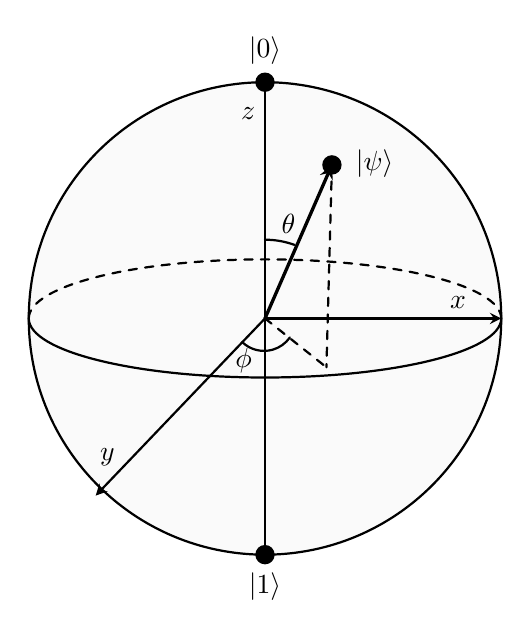
\begin{tikzpicture}[
            scale=1,
            line cap=round,
            line join=round,
            >=stealth
        ]
    
        % Sphere
        \def\R{3}
        \draw[thick, fill=gray!4] (0,0) circle (\R);
    
        % Equator: hidden rear half and visible front half
        \draw[thick]
            (-\R,0) arc[start angle=180,end angle=360,
                        x radius=\R,y radius=0.75];
    
        \draw[thick, dashed]
            (\R,0) arc[start angle=0,end angle=180,
                        x radius=\R,y radius=0.75];
    
        % Coordinate axes
        \draw[thick] (0,0) -- (0,3);
        \draw[thick] (0,0) -- (0,-3);
    
        \draw[thick,->] (0,0) -- (-2.15,-2.25);
        \node[above] at (-2,-2) {$y$};
        \draw[thick,->]    (0,0) -- (3,0);
        \node[above] at (2.45,0) {$x$};
        \node[left] at (0,2.6) {$z$};
    
        % Bloch vector endpoint and its projection
        \coordinate (P) at (0.85,1.95);
        \coordinate (Q) at (0.78,-0.62);
    
        \draw[very thick,->] (0,0) -- (P);
        \fill (P) circle (3.5pt);
    
        % Dashed projection onto the equatorial plane
        \draw[thick,dashed] (P) -- (Q);
        \draw[thick,dashed] (0,0) -- (Q);
    
        % Polar angle theta
        \draw[thick]
            (0,1)
            arc[start angle=90,end angle=70,radius=1.1];
    
        \node at (0.3,1.2) {$\theta$};
    
        % Azimuthal angle phi
        \draw[thick]
            (-0.29,-0.3)
            arc[start angle=226,end angle=325,
                radius=0.4];
    
        \node at (-0.27,-0.53) {$\phi$};
    
        % Basis-state labels
        \fill (0,3) circle (3.5pt);
        \fill (0,-3) circle (3.5pt);
    
        \node[above] at (0,3.1) {$\ket{0}$};
        \node[below] at (0,-3.1) {$\ket{1}$};
    
        % State label
        \node[right] at ($(P)+(0.18,0.02)$) {$\ket{\psi}$};
    
        \end{tikzpicture}
    \end{center}
    The Bloch sphere is useful because it turns a two-level quantum state into geometry: measurement probabilities become projections, unitary evolution becomes rotation, and mixedness becomes distance from the center.
    \subsection{Visualizing a state as a point on the sphere}
    Choose \(|0\rangle=|\uparrow\rangle\) and \(|1\rangle=|\downarrow\rangle\). Any normalized pure qubit state, after removing an overall phase, can be written as
    \[
    |\psi\rangle=\cos\left(\tfrac{\theta}{2}\right)|0\rangle
    +e^{i\phi}\sin\left(\tfrac{\theta}{2}\right)|1\rangle
    \]Its Bloch vector is
    \[
    {\mathbf r=(\sin\theta\cos\phi,\;\sin\theta\sin\phi,\;\cos\theta).}
    \]
    which is the unit radial vector in spherical coordinates. Here \(\theta\) is the polar angle measured from \(+z\), and \(\phi\) is the azimuthal angle. \\ \\
    The half-angle in the ket makes it so that
    \begin{enumerate}[label=(\roman*)]
        \item \(|0\rangle\) and \(|1\rangle\) are the north and south poles
        \item \((|0\rangle\pm|1\rangle)/\sqrt2\) point along \(\pm x\)
        \item \((|0\rangle\pm i|1\rangle)/\sqrt2\) point along \(\pm y\)
        \item The Pauli expectations are equal to the cooresponding coordinate of the Bloch vector i.e. the projection onto the $x,y,z$ axes
        \begin{align*}
            \langle X\rangle=\sin\theta\cos\phi\qquad,\qquad\langle Y\rangle = \sin\theta\sin\phi\qquad,\qquad\langle Z\rangle=\cos\theta
        \end{align*}
    \end{enumerate}
    Orthogonal kets correspond to antipodal points on the sphere, not perpendicular Bloch vectors. Multiplying a ket by an overall phase leaves its point unchanged while changing the relative phase moves it. \\ \\
    Other useful facts:
    \begin{enumerate}[label=(\roman*)]
        \item $\theta$ controls the measurement probabilies in the $z$-basis i.e.
        \begin{align*}
            P(Z=+1)=\cos^2(\theta/2)\qquad,\qquad P(Z=-1)=\sin^2(\theta/2)
        \end{align*}
    \end{enumerate}
\end{document}